%% This is an example first chapter.  You should put chapter/appendix that you
%% write into a separate file, and add a line \include{yourfilename} to
%% main.tex, where `yourfilename.tex' is the name of the chapter/appendix file.
%% You can process specific files by typing their names in at the 
%% \files=
%% prompt when you run the file main.tex through LaTeX.
\chapter{Introducción}\label{intro_secc}

El filtrado y procesamiento de imágenes es utilizado en múltiples campos, como
la medicina, ingeniería, navegación, aeronáutica, entre otros. En el campo de la
inteligencia artificial, área emergente que es de mero interés hoy en día, la
convolución en 2D es la operación principal que se realiza en una CNN (Red
neuronal Convolucional)~\cite{Lecun-et-al-1998}.

Dada su naturaleza, la operación de convolución en 2-D es la más empleada en los
algoritmos de procesamiento de imágenes. El paralelismo inherente de algoritmos
basados en la convolución es explotado logrando alta performance en estos
sistemas que los utilizan.

La convolucion bidimensional, se define matemáticamente como:
\begin{equation}\label{conv-org}
  G(x,y) = \sum_{i=0}^{m-1} \sum_{j=0}^{n-1}K(i,j)I(x-i,y-j)
\end{equation}
Donde $I(x,y)$ es una imagen de $(m \times n)$ pixels, $K(i,j)$ un conjunto de
coeficientes denominado kernel, de tamaño $(k \times k)$ and $G(x,y)$ es la
convolucion resultante de tamaño  $(m-2 \times n-2)$ pues se considera una
\textit{valid convolution}~\cite{validconv}. 

El uso de Field Programmable Gate Arrays (FPGAs) para implementar este tipo de
sistemas, se debe a la ventaja que presentan estos dispositivos en lo que
concierne al paralelismo a nivel bit, pixel, vecindad y a nivel tarea, lo
incrementa la performance y velocidad de cómputo.~\cite{papercnn}

Existen múltiples ejemplos en la literatura de implementaciones de convolución
2D. Como se muestra en~\cite{paper3}, la BRAM es uno de los elementos
mas usados con el consumo de energía mas alto. Las arquitecturas que se
encuentran se pueden clasificar en dos grupos, aquellas que consideran un
almacenamiento total de la imagen~\cite{paper1, paper5} y las que consideran un
almacenamiento parcial donde la imagen se particiona en
segmentos~\cite{paper2,paper4}. El problema que se encuentra en estos esquema es
la falta de modularización del procesamiento, lo que dificulta mejorar la frecuencia
de trabajo incrementado el paralelismo.

En este trabajo presentamos el concepto del reuso dinámico de BRAM en
convolución 2D y la complejidad de su implementación para arquitecturas con
paralelismo. Además, proponemos una arquitectura modular que facilita la
escalabilidad.

\section{Preprocesamiento}\label{dynamicrange}

Los pixeles de la imagen en escala de grises $I(x,y)$ tienen un rango dinámico
de valores que se hallan entre $[0,255]$, y los valores que toma el kernel
$K(x,y)$ pueden ser positivos o negativos.

Dado que el sistema desarrollado forma parte de un proyecto de Deep Learning,
donde es usual operar en un rango dinámico centrado en cero, se aplicó una
transformación denominada  expansión dinámica de rango\cite{dinamic_rango} ($\mathcal{D}([.])$),
junto con Maximum Norm\cite{max_norm} ($(\mathcal{M}[.])$) para reacomodar los diferentes 
rangos de valores. Más sobre esto en la sección siguiente.

Para el caso de la imagen, se tiene $\mathcal{D}[I(x,y)]=I^\prime(x,y)$ y un
rango resultante de $[0,1]$. Para el caso del kernel,
$\mathcal{M}[K(x,y)]=K^\prime(x,y)$ con un rango $[-1,1]$, respectivamente.
Así, reemplazando en la ecuación~\ref{conv-org}, se tiene 
\begin{equation}\label{conv-org1}
  G(x,y) = \mathcal{D}^{-1}\left[\sum_{i=0}^{m-1} \sum_{j=0}^{n-1}K^\prime(i,j)I^\prime(x-i,y-j)\right],
\end{equation}
siendo $\mathcal{D}^{-1}[.]$ el cambio de rango dinamico entre $[0,255]$.

La figura~\ref{transformation} muestra el proceso completo de mapeo de datos, se
aplica la transformación a la imagen de entrada, luego se convoluciona con el
kernel y se hace la transformación inversa a ese resultado para volverlo a
mapear al conjunto de valores iniciales.

\begin{figure}
\centering
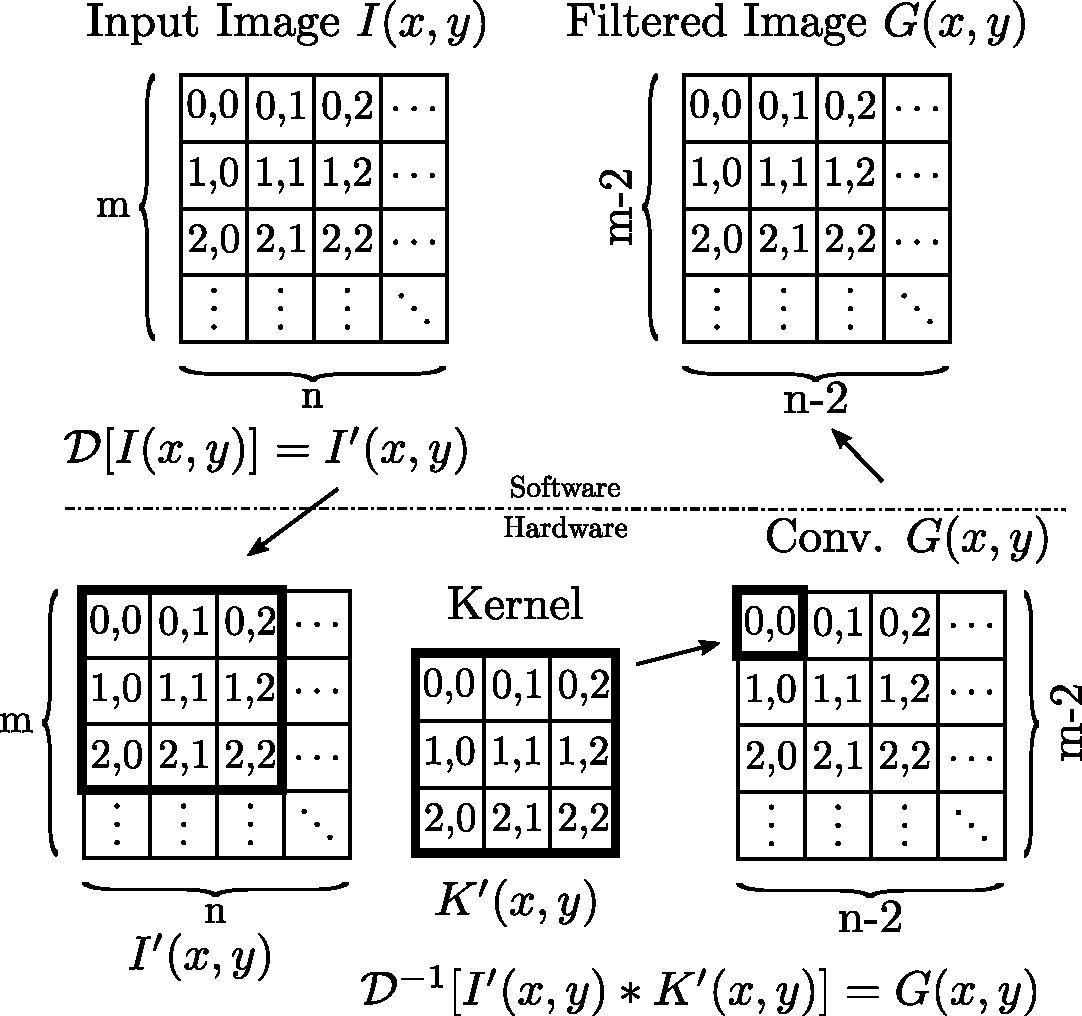
\includegraphics[scale=0.5]{wflow3}
\caption{Transformaciones del rango dinámico durante el procesamiento de la imagen.}
\label{transformation}
\end{figure}

\section{Representación en punto fijo}\label{fixedpoint}

La representación en punto flotante, almacena los números en términos de la
mantisa y del exponente. El hardware que soporta el formato punto flotante,
luego de ejecutar cada computo, automáticamente escala la mantisa y actualiza el
exponente para que el resultado se corresponda con el número de bits de forma
definida. Todas estas operaciones hacen que el hardware que soporte punto
flotante, sea más costoso en términos de área y potencia. Emerge una
alternativa: la representación en punto fijo.

La representación en punto fijo se emplea para
almacenar y manipular datos, con cierto número de bits fijos. Esto implica que
luego del cómputo, no se sigue la posición del punto decimal, y se le delega
esta responsabilidad al diseñador del hardware. El punto decimal, valga la
redundancia, es fijo para cada variable, y es predefinido. Fijando el punto, una
variable se limita a tomar un rango fijo de valores. Pese a que este límite nos
brinda ventajas en lo que refiere a utilización de recursos, si el resultado del
cómputo cae fuera del rango, se produce un overflow. Existen varias formas de
manipular los overflows que emergen como resultado de un cómputo en punto fijo
(redondeo, saturación, truncamiento) y sigue siendo responsabilidad del
diseñador optar por la representación adecuada según el sistema que pretende
llevar a cabo.

Este an\'alisis tiene por objeto el trabajar con una m\'inima representaci\'on
finita para los p\'ixeles de la imagen y los valores del kernel.
Para ello se necesita efectuar un estudio acerca de la cantidad de bits de
resoluci\'on m\'inimos  con una p\'erdida de informaci\'on aceptable.

Como se nombro anteriormente, los valores de los p\'ixeles \(I_{ij}\) se
encuentran en el rango 0 a 255. Con la normalización dynamic range
expansion se los lleva al rango 0 a 1. Los valores del kernel
\(K_{ij}\) pueden ser tanto positivos como negativos. Utilizando Maximum
norm se lleva al kernel al rango -1 a 1.

Para poder operar los rangos anteriores en una representaci\'on de 8 bits se
utiliza representac\'ion Signed Fixed Point\cite{fix_p} \(S(8,7)\). 

La convoluci\'on de una imagen con un $K^{3{\times}3}$ resulta en una 
salida de 20 bits, en \(S(16,14)\) por cada producto sumado la adici\'on de los nueve
elemento tiene una representaci\'on total de \(S(20,14)\).Entonces se realiza un
post procesamiento donde se lleva el resultado a un rango positivo y truncamiento.
Se establece una comparaci\'on a fines de decidir la cantidad de bits de salida del
procesamiento.

Para realizar una comparaci\'on se utiliza la relaci\'on SNR de la operaci\'on a
m\'axima resoluci\'on \(S(20,14)\) y el error producido al reducir la cantidad
de bits ${e_r=f(x)_{20b}-f(x)_{pos}}$\cite{srntesis}.

\begin{figure}
\centering
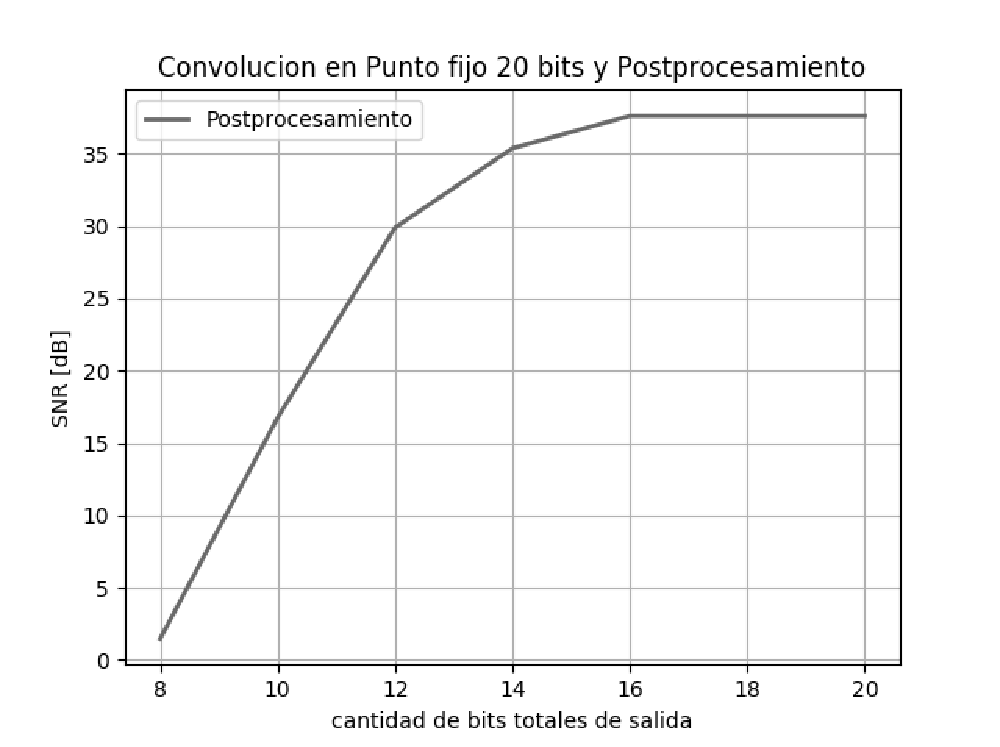
\includegraphics[scale=0.47]{posprocesamiento2}
\caption{Nivel de error según la resolución en bits.}
\label{prepro}
\end{figure}

Al la convolucionar con un filtro unitario y realizar una reducci\'on de los
bits de la parte fraccionaria, partiendo de 8 bits en totales, mejora la
representaci\'on de la imagen , y que a partir de 13 bits totales 1 bit de
signo, 5 bits parte entera y 7 en parte fraccionaria, con una representación
\(S(13,8)\) tiene una SNR aprimada de \(30 [dB]\) que permite observar el efecto
de la convolucion con una m\'inima perdida de informaci\'on recordando que
nuestro objetivo no es no es representar una imagen en su totalidad.

\begin{figure}[!t]
  \centering
  \subfloat{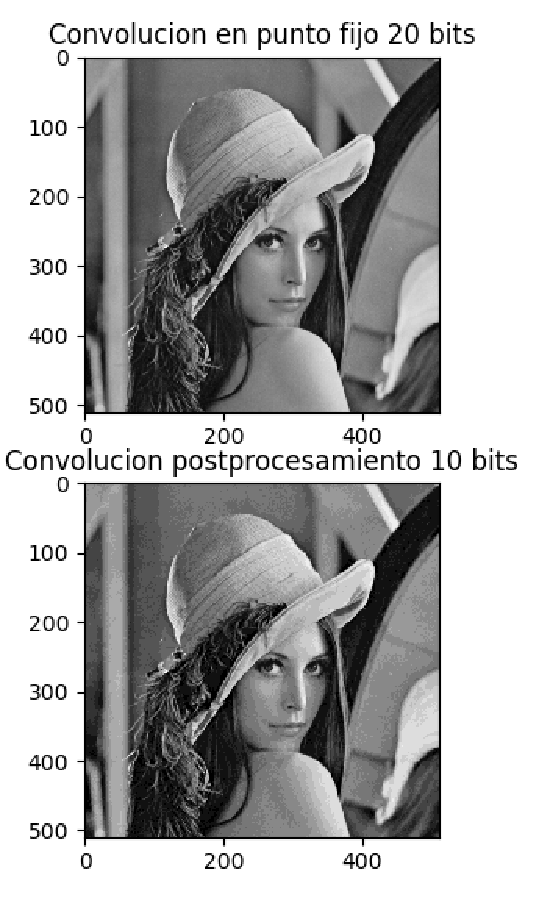
\includegraphics[scale=0.5]{posprocesanto1}}%
    \hfil %\vspace{0.1cm}
    \centering
    \subfloat{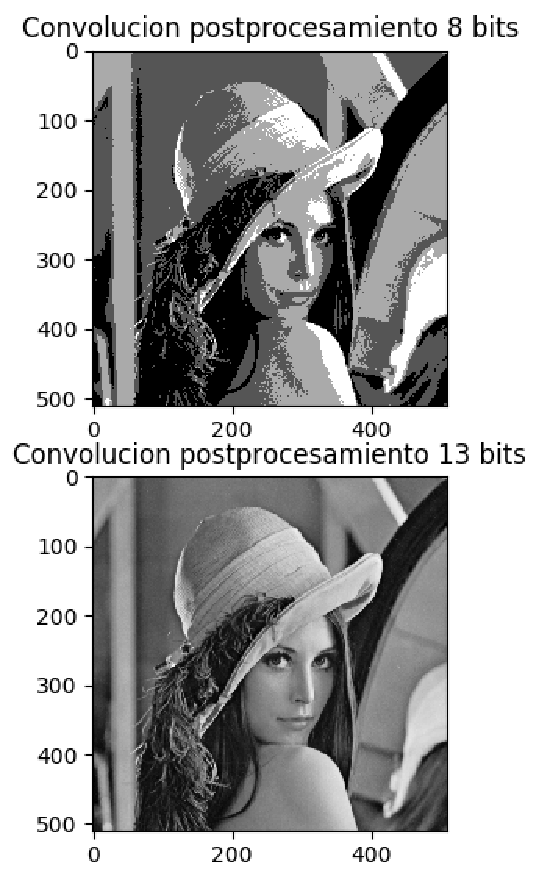
\includegraphics[scale=0.5]{posprocesanto2}}%
      \caption{Degradación de la imagen según la resolución en bits.}
      \label{prepro2}
    \end{figure}

Se puede llevar el rango final a 8 bits si se utiliza dynamic range expansion.
Pero se requiere conocer el m\'aximo y el m\'inimo valor de p\'ixel de la imagen
luego de filtrar, lo que implica que toda la imagen se encuentre en memoria.

\section{Flujo de diseño} \label{flujo_subsecc}

Se estructuró el proyecto y se siguió el flujo o estructura de la
Fig.~\ref{design_flow} para llevar el proyecto a cabo en el tiempo disponible.

En primera instancia se partió de las especificaciones, simulando el comportamiento en punto flotante mediante el lenguaje de alto nivel Python. Luego, se analizaron los resultados obtenidos tras implementar el sistema en punto fijo, a nivel software. 
Fijados los requerimientos se comenzó con el diseño del hardware,
previamente habiendo estudiado y modelado la arquitectura del sistema, la cual
se detalla en la seccion \ref{arquitectura_sec}.

\begin{figure}
\centering
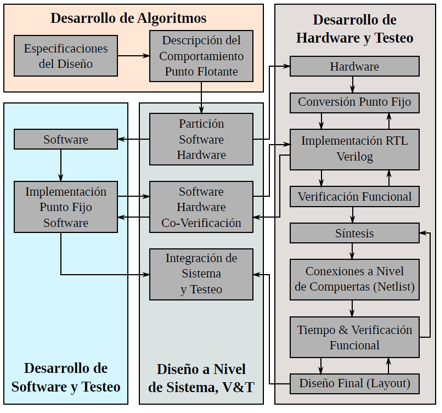
\includegraphics{flujo_de_dis.png}
\caption{Esquemático del flujo de diseño seguido.}
\label{design_flow}
\end{figure}

\subsection{Testing}

Se realizaron diferentes tipos de testing: test
unitarios de cada módulo (test bench del módulo), test de integración (varios
módulos y su interacción) y finalmente test de sistema, donde se probó el
funcionamiento del sistema completo dada cierta imagen de entrada. Para realizar
el proceso de testeo, en primera instancia se corrobora que los bits producidos
por el simulador del hardware descripto coincidieran con los bits del simulador
del sistema en Python, una vez pasada esta etapa con éxito, se implementa el
hardware en una FPGA y se comprueba nuevamente que los resultados obtenidos no
difieran con los simulados.